% Pontos A(0,0), B(2,3), C(6,3), D(6,0)
% Apoio fixo em A, apoio móvel em D
% 20kN/m entre (0,3) e (6,3)
% Carga triangular de 0 a 16kN/m entre C e D

\documentclass[tikz]{standalone}
\usepackage{stanli}
\usetikzlibrary{calc}

\begin{document}
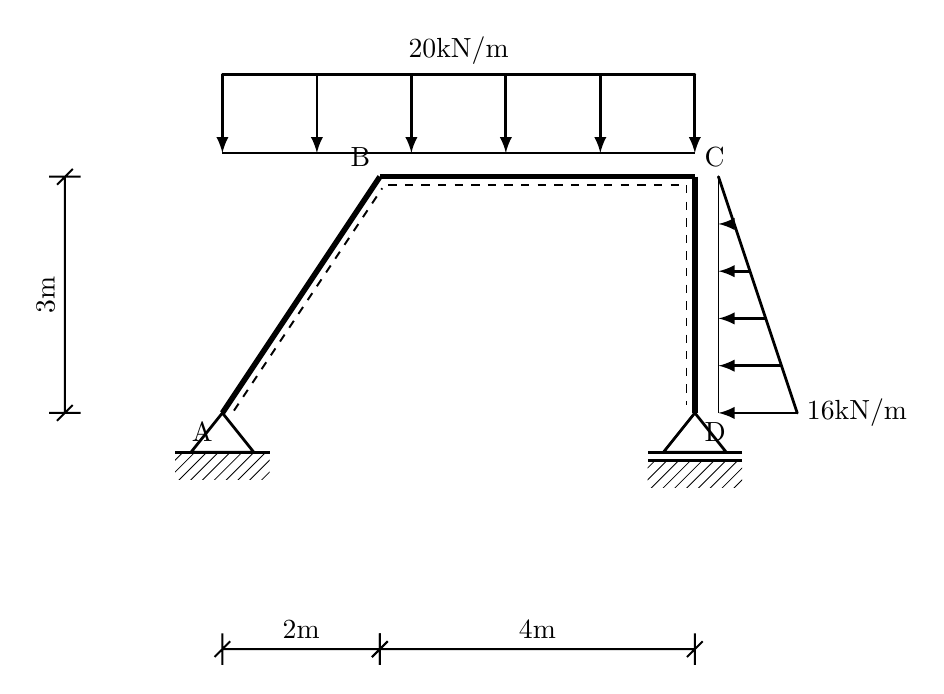
\begin{tikzpicture}
    % Definição dos pontos principais
    \point{A}{0}{0}
    \point{B}{2}{3}
    \point{C}{6}{3}
    \point{D}{6}{0}
    
    % Ponto auxiliar para o início da carga distribuída (conforme coordenadas (0,3))
    \point{L}{0}{3}

    % Definição dos apoios
    \support{1}{A} % Apoio fixo
    \support{2}{D} % Apoio móvel

    % Definição das barras do pórtico
    \beam{1}{A}{B}
    \beam{1}{B}{C}
    \beam{1}{C}{D}

    % Cargas
    % Carga uniformemente distribuída de 20kN/m entre (0,3) e (6,3)
    \lineload{1}{L}{C}
    
    % Carga triangular de 0 a 16kN/m entre C e D (normal à barra vertical)
    % Usamos [0][1] para definir o gradiente de 0% a 100% da carga
    \lineload{1}{C}{D}[0][1]

    % Notações e Etiquetas
    \notation{1}{A}{A}[below left]
    \notation{1}{B}{B}[above left]
    \notation{1}{C}{C}[above right]
    \notation{1}{D}{D}[below right]
    
    % Rótulo da carga de 20kN/m (Regra: above=13mm)
    \notation{5}{L}{C}[20kN/m][.5][above=13mm]
    
    % Rótulo da carga triangular de 16kN/m no ponto de intensidade máxima (D)
    \notation{1}{D}{16kN/m}[right=13mm]

    % Dimensionamento
    % Horizontal (distância negativa para ficar abaixo dos apoios)
    \dimensioning{1}{A}{B}{-30mm}[2m]
    \dimensioning{1}{B}{C}{-30mm}[4m]
    
    % Vertical (distância negativa para ficar à esquerda da estrutura)
    \dimensioning{2}{A}{B}{-20mm}[3m]
    
\end{tikzpicture}
\end{document}